\label{sec:modeling}
We restrict ourselves to considering the swimmer \textsc{Spr4} proposed in \cite{Alouges2013}. Let $(S_1, S_2, S_3, S_4)$ be a regular reference tetrahedron centered at $c \in \R^3$ such that $\dist(c, S_i) = 1$ for all $i \in \N_4$. Then the swimmer consists of four balls $(B_i)_{i \in \N_4}$ of $\R^3$ centered at $b_i \in \R^3$, all of radius $a > 0$, such that the ball $B_i$ can move along the ray starting at $c$ and passing through $S_i$, see figure \ref{fig:reference tetrahedron and spr4}.

\begin{figure}[h]
    \centering
    \begin{minipage}{0.45\textwidth}
        \centering
        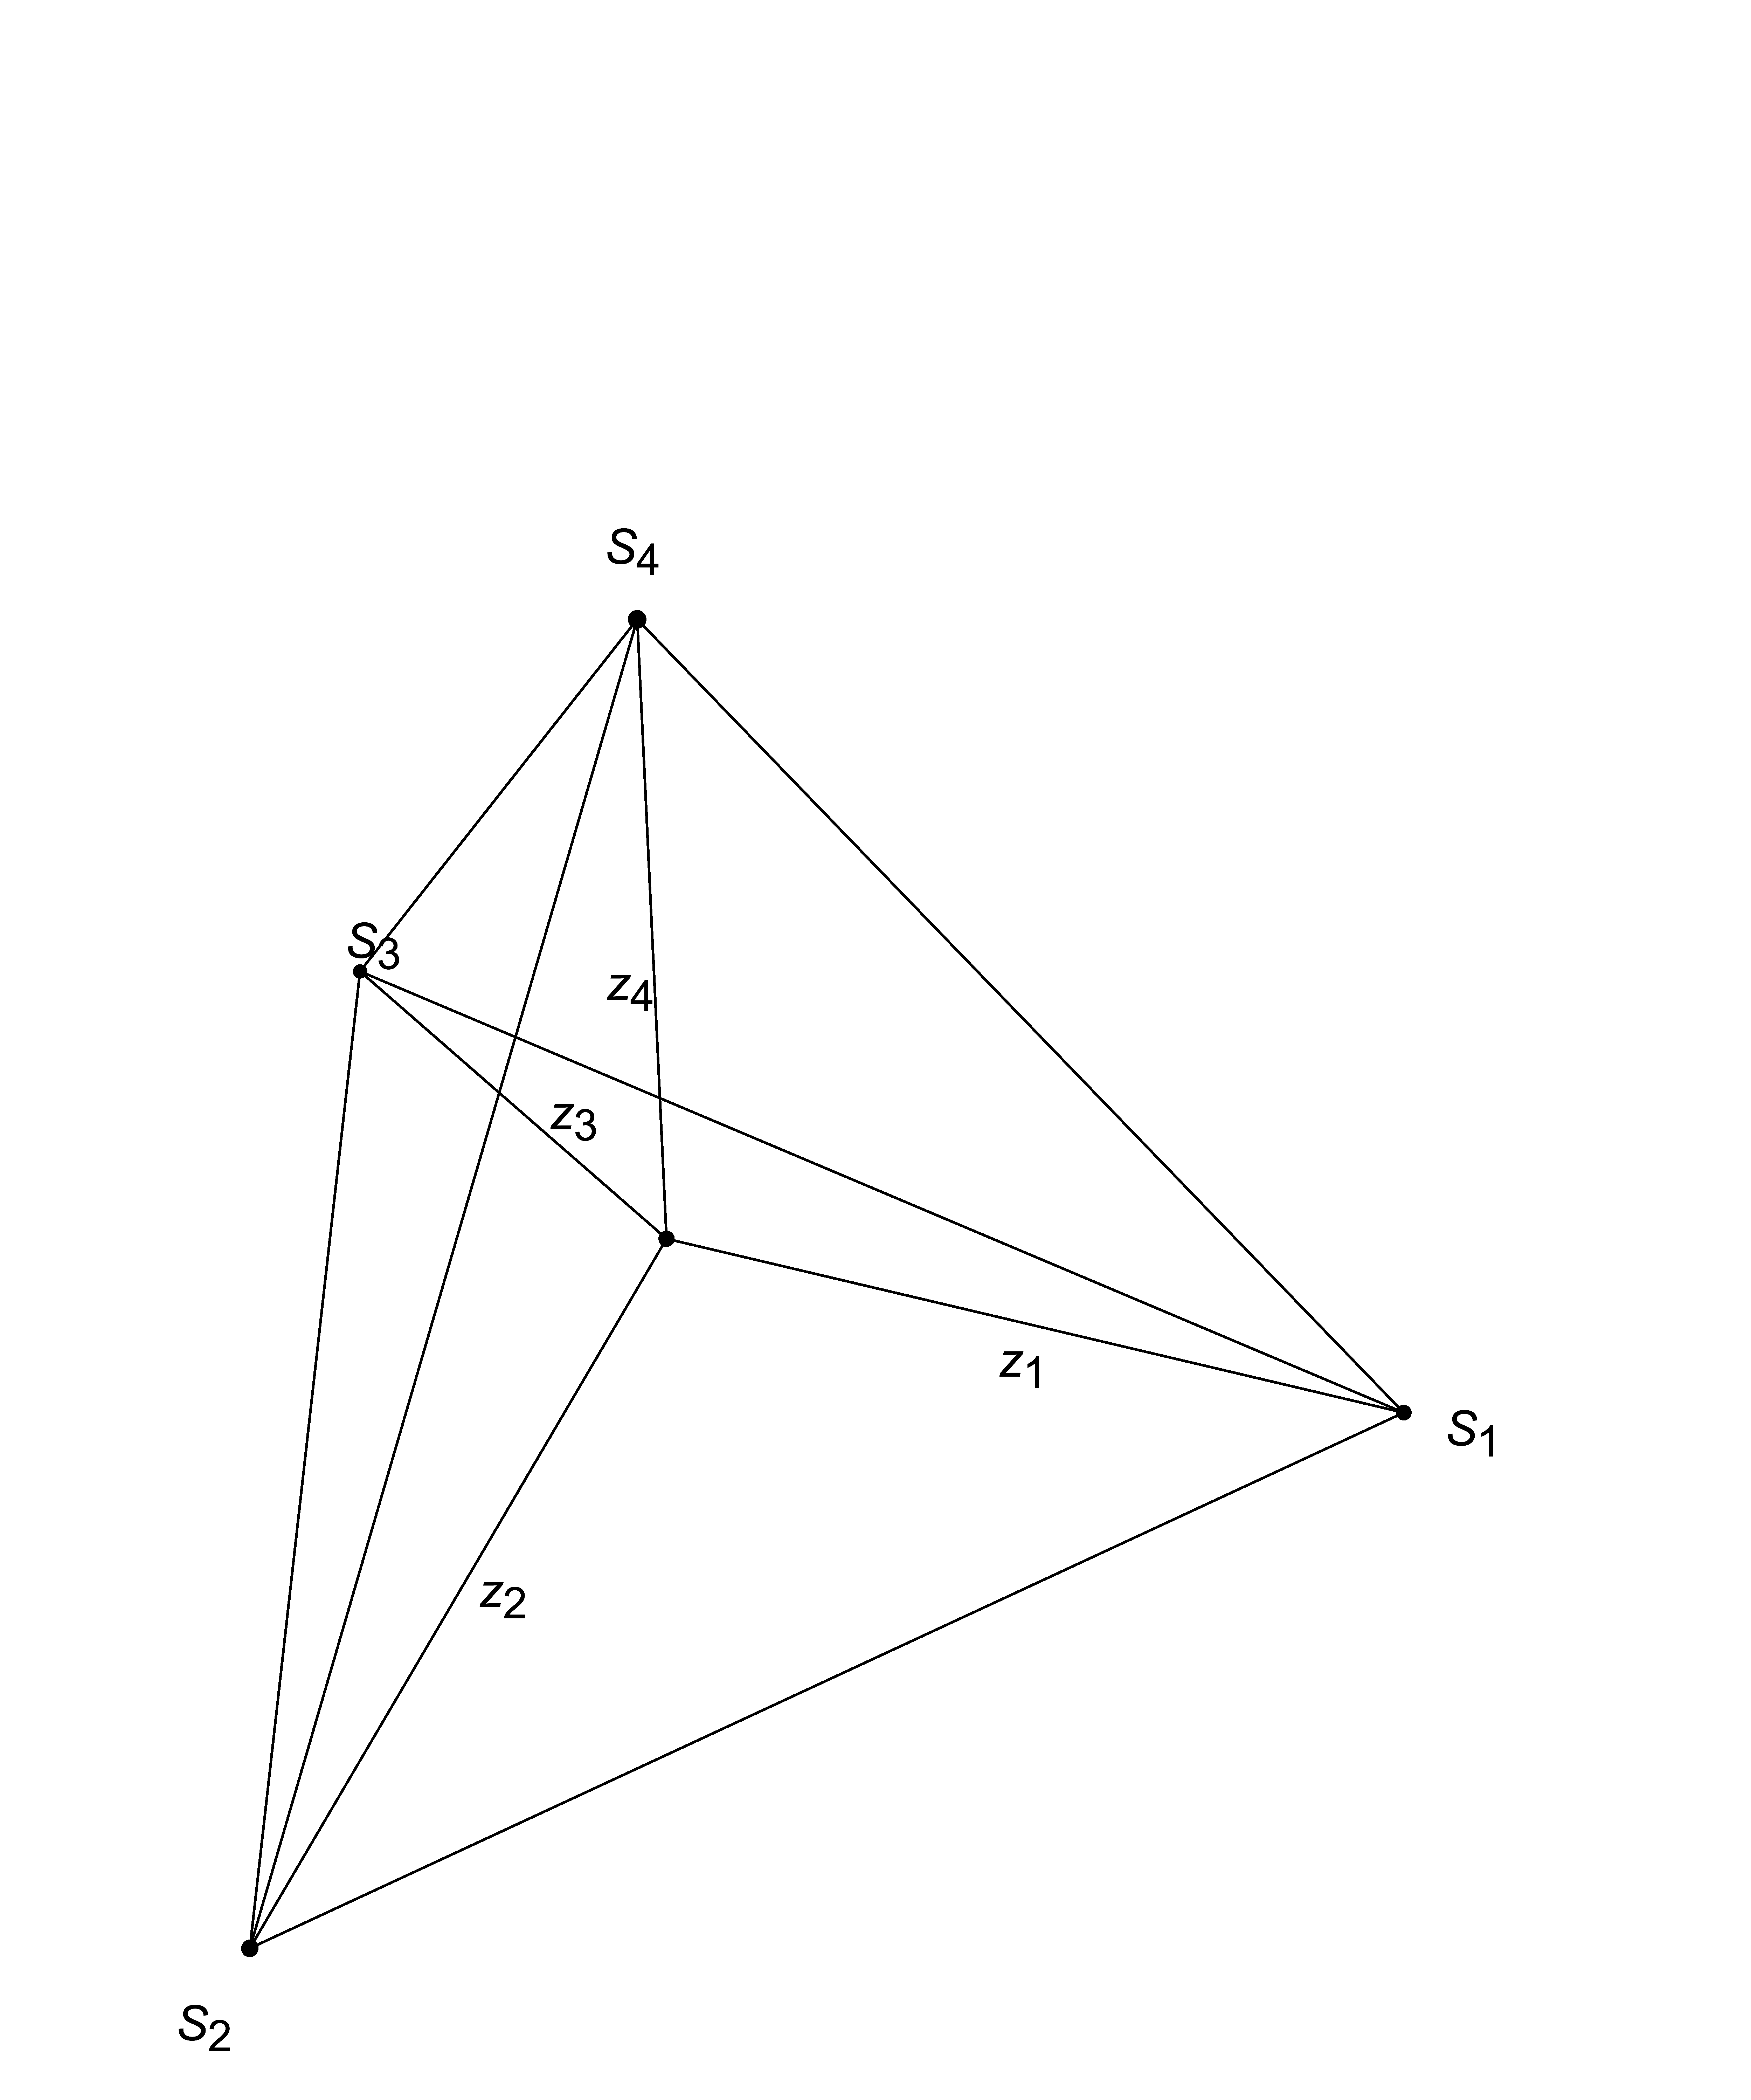
\includegraphics[width=0.9\textwidth]{/Users/philipp/Documents/GitHub/stage_cmap/images/tetrahedron.png}
    \end{minipage}
    \begin{minipage}{0.45\textwidth}
        \centering
        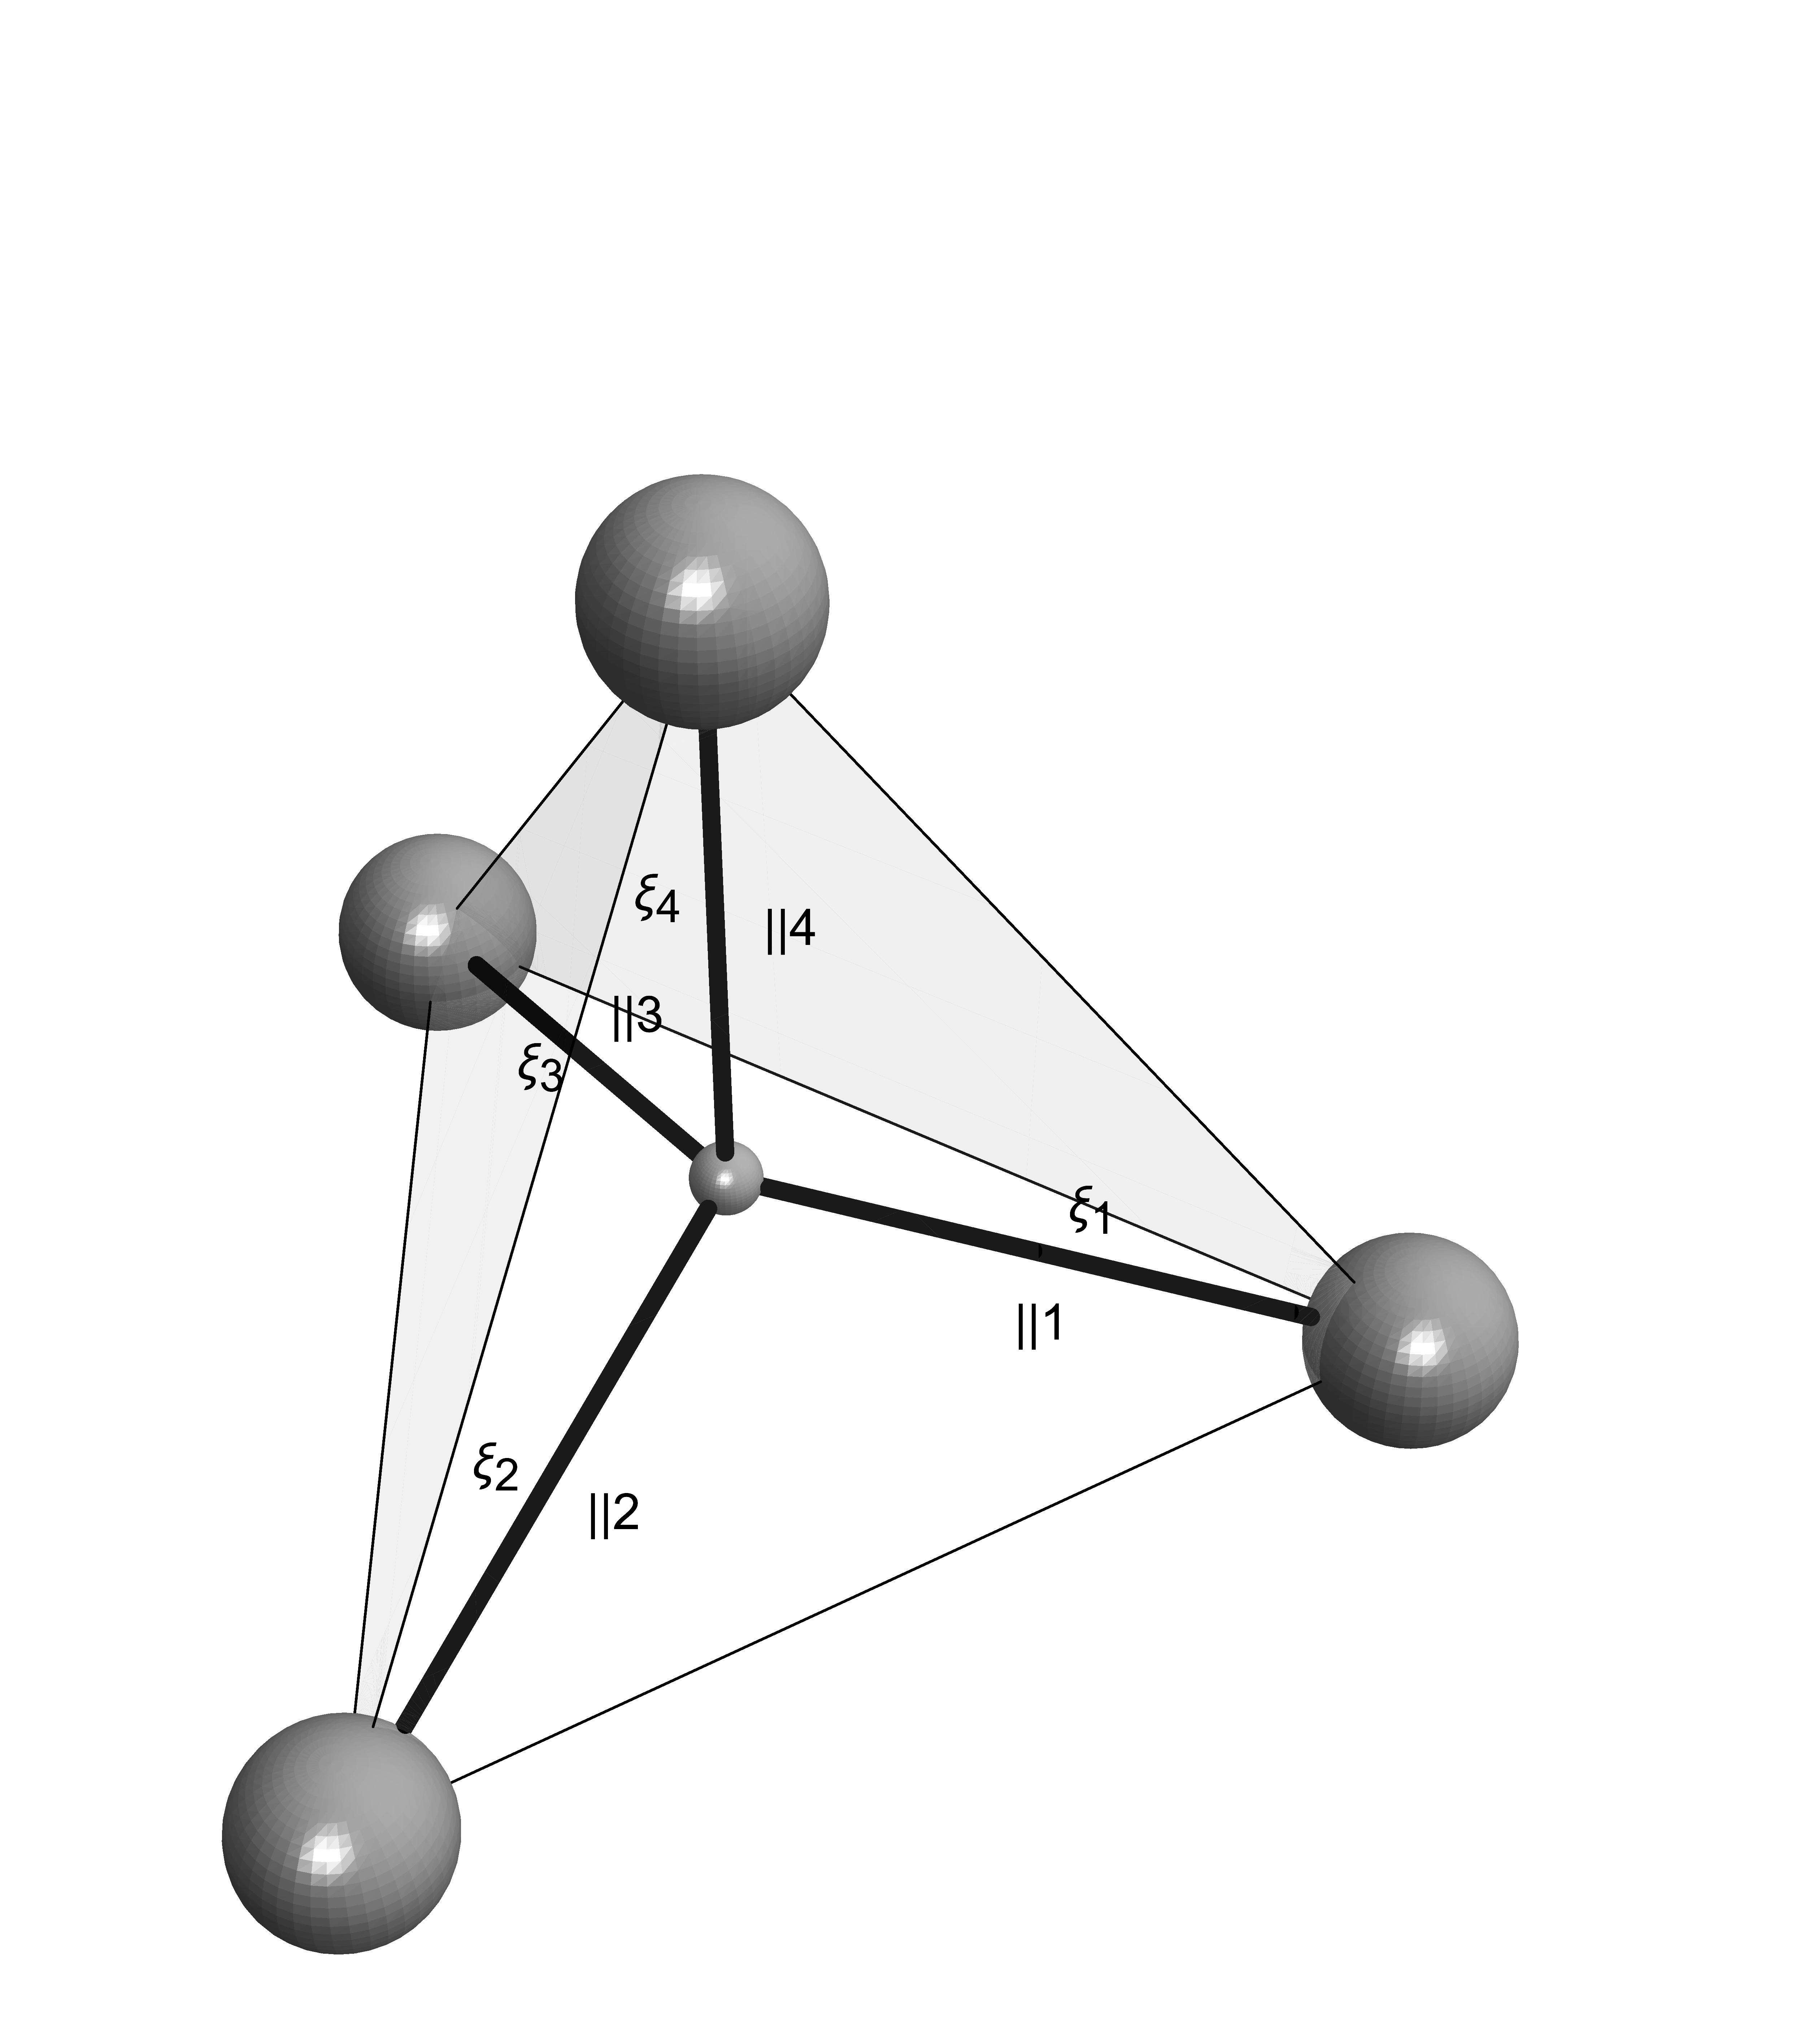
\includegraphics[width=0.9\textwidth]{/Users/philipp/Documents/GitHub/stage_cmap/images/spr4.png} % second figure itself
    \end{minipage}
    \caption{The reference tetrahedron and the parking 4-sphere swimmer (\textsc{SPr4}).}
    \label{fig:reference tetrahedron and spr4}
\end{figure}

 This reflects the situation where the balls are linked together by thin jacks that are able to elongate and retract. However, the viscous resistance of these jacks is neglected and therefore the fluid is assumed to permeate the entire open set $\R^3 \setminus \bigcup_{i = 1}^{4} \overline{B}_i$. The balls do not rotate around their arms which implies that the shape of the swimmer is completely determined by the four lengths $\xi_1, \xi_2, \xi_3, \xi_4$ of its arms, measured from $c$ to the center of each ball $b_i$. However, there are no restrictions for the rotation of the swimmer around the center $c$, i.e. for fixed arm lengths, the swimmer is considered to be a rigid body in a Stokesian fluid.
Hence, the geometrical configuration of the swimmer can be described by two sets of variables:
\begin{enumerate}
	\item The vector of \emph{shape variables} $\xi := (\xi_1, \xi_2, \xi_3, \xi_4) \in \M := (\sqrt{\tfrac{3}{2}}a, +\infty)^4 \subseteq \R_+^4$, from which one obtains the relative distances $(b_{ij})_{i,j \in \N_4}$ between the balls,  where the lower bound in the open intervals is chosen such that the balls cannot overlap.
	\item The vector of \emph{position variables} $p = (c, R) \in \mathcal{P} :=  \R^3 \times \SO(3)$, which encodes the global position and orientation in space of the swimmer.
\end{enumerate}
To be more precise, we consider the reference tetrahedron convexly spanned by the four unit vectors $z_1 := (2 \sqrt{2}/3,0,-1/3)$, $z_2 := (-\sqrt{2}/3,-\sqrt{2/3},-1/3)$, $z_3 := (-\sqrt{2}/3,\sqrt{2/3},-1/3)$ and $z_4 := (0,0,1)$. Position and orientation in $\R^3$ are then described by the coordinates of the center $c \in \R^3$ and the rotation $R \in SO(3)$ of the swimmer with respect to the reference orientation induced by the reference tetrahedron, i.e. if the arms are aligned with the reference tetrahedron, then this corresponds to the identity matrix $I \in \SO(3)$. Thus, we set $b_i := c + \xi_i R z_i$ for the center of the ball $B_i$.

The swimmer is completely described by the parameters $(\xi, p) \in \M \times \mathcal{P}$. Indeed, if we denote by $B_a$ the ball in $\R^3$ of radius $a$ centered at the origin, then for any $r \in \partial B_a$, the position of the current point on the $i$-th sphere of the swimmer in the state $(\xi, p)$ is given, for any $(\xi, p, r) \in \M \times \mathcal{P} \times \partial B_a$, by the function
\begin{equation}
	r_i(\xi, p, r) :=  c + R(\xi_i z_i + r).
\end{equation}
Note that the functions $(r_i)_{i \in \N_4}$ are analytic in $\M  \times \mathcal{P}$ and thus we can use them to calculate the instantaneous velocity on the $i$-th sphere $B_i$, which for any $(\xi, p, r) \in \M \times \mathcal{P} \times \partial B_a$ and every $i \in \N_4$ is given by
\begin{equation}
	u_i(\xi, p, r) = \dot{c} + \omega \times (\xi_i z_i + r) + R z_i \dot{\xi}_i,
\end{equation}
where $\omega$ is the axial vector associated with the skew matrix $\dot{R} R$.

In \cite{Alouges2013} it is shown that the system \textsc{SPr4}, i.e. both the shape $\xi$ and the position $p$, is controllable only using the rate of change $\dot{\xi}$ of the shape. To do so, we have to understand how $p$ responds to a variation in $\dot{\xi}$. To that end, the assumptions of \emph{self-propulsion} and \emph{negligible inertia of the swimmer} (which is equivalent to assuming a very low Reynolds number) are made. They imply that the total viscous force and torque exerted by the surrounding fluid on the swimmer must vanish. More precisely, for details see \cite{Alouges2013}, the system can be written as
\begin{equation}
\label{eq: control system}
	\dot{p} = F(R, \xi) \dot{\xi} := \left ( \begin{array}{c}
	F_c(R, \xi) \\
	F_\theta(R, \xi)
	\end{array}  \right ) \dot{\xi},
\end{equation}
where $\dot{c} = F_c(R, \xi) \dot{\xi}$ and $\dot{R} = F_\theta (R, \xi) \dot{\xi} $. 

In preparation for what follows, let us note that if we denote by $T_p \mathcal{P}$ the tangent space of the smooth manifold $\mathcal{P}$ at the point $p$, we have $F(R, \xi) \in \mathcal{L}(\R^4, T_{p}\mathcal{P})$ for any $R \in \SO(3)$ and $\xi \in \R^4$, where $\mathcal{L}(V, W)$ denotes the linear maps between two vector spaces $V$ and $W$. We quickly recall the fact that at any point $R \in \SO(3)$, see e.g. \cite{Hall2015} for details, we have 
\begin{equation}
	T_R \SO(3)  = \{R M \mid M \in \Skew_3(\R)\},
\end{equation}
where $\Skew_n(\R)$ denotes the set of skew-symmetric real matrices of size $n \times n$. Hence, we have in particular that for any $R \in \SO(3)$ and $\xi \in \R^4$
\begin{equation}
\begin{aligned}
	F_c(R, \xi) \in \mathcal{L}(\R^4, \R^3) \text{ and } F_{\theta}(R, \xi) \in \mathcal{L}(\R^4,T_R \SO(3))
\end{aligned}
\end{equation}
and therefore we can express both $F_c(R, \xi)$ and $F_{\theta}(R, \xi)$ as real matrices of size $3 \times 4$ once we have chosen a basis for the corresponding tangent spaces. Indeed, one verifies quickly that $\Skew_3(\R)$ is a three-dimensional vector space over $\R$.


 In analogy to \cite{Alouges2017}, it is important to note here that the control system $F$ is independent of $c$ due to the translational invariance of the Stokes equations. However, the translational invariance is not the only symmetry property that \textsc{SPr4} satisfies. The goal of the following section is to examine the structure of the control system $F$ in consequence of the symmetries it must fulfill being driven by the Stokes equations.





























